\documentclass{scrreprt}
%\usepackage{float}
\usepackage{fullpage}
\usepackage{caption}
\usepackage{subcaption}
\usepackage{listings}
\usepackage{underscore}
\usepackage{tabularx}
\usepackage{longtable}
\usepackage{graphicx}
\usepackage[bookmarks=true]{hyperref}
\usepackage{pdfpages}
\usepackage{cite}

\setcounter{secnumdepth}{3}
\setcounter{tocdepth}{3}

\definecolor{airforceblue}{rgb}{0.66, .0, 0.36}

\hypersetup{
%    bookmarks=false,    % show bookmarks bar?
    pdftitle={Software Requirement Specification},    % title
    pdfauthor={Homer J. Simpson},                     % author
    pdfsubject={TeX and LaTeX},                        % subject of the document
    pdfkeywords={TeX, LaTeX, graphics, images}, % list of keywords
    colorlinks=true,       % false: boxed links; true: colored links
    linkcolor=blue,       % color of internal links
    citecolor=black,       % color of links to bibliography
    filecolor=black,        % color of file links
    urlcolor=purple,        % color of external links
    linktoc=page            % only page is linked
}

\def\myversion{1.0 }

\newcounter{myCounter}[subsubsection] 
\newcounter{mySubCounter}[myCounter] 

\makeatletter
\newcommand{\reqLabel}[1]{%
\myLabel{#1}{Req}}
\makeatother

\makeatletter
\newcommand{\reqLabelB}[1]{%
\myLabelB{#1}{Req}}
\makeatother

\makeatletter
\newcommand{\specLabel}[1]{%
\myLabel{#1}{Spec}}
\makeatother

\makeatletter
\newcommand{\specLabelB}[1]{%
\myLabelB{#1}{Spec}}
\makeatother

\makeatletter
\newcommand{\defLabel}[1]{%
\myLabel{#1}{Def}}
\makeatother

\makeatletter
\newcommand{\nfLabel}[1]{%
\myLabel{#1}{NF}}
\makeatother

\makeatletter
\newcommand{\rightMouse}{%
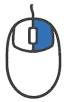
\includegraphics[width=15pt]{img/rightMouse.png}}
\makeatother

\makeatletter
\newcommand{\rightArrow}{%

\includegraphics[width=10pt]{img/rightArrow.jpeg}\hspace{1mm}}
\makeatother

%%%%%%%%%%%%%%%%%%%%%%%%%%%%%%%%%% Variante 1 %%%%%%%%%%%%%%%%%%%%%%%%%%%%%%%%%%%%%%%
\newcommand{\layerOne}[1]{\chapter{#1}}
\newcommand{\layerOneStar}[1]{\chapter*{#1}}
\newcommand{\layerTwo}[1]{\section{#1}}
\newcommand{\layerThree}[1]{\subsection{#1}}
\newcommand{\layerFour}[1]{\subsubsection{#1}}

\makeatletter
	\newcommand{\myLabel}[2]{%
		\refstepcounter{myCounter}
		\def\@currentlabel{#2-\thesubsubsection.\arabic{myCounter}}% Update label
		\raisebox{\f@size pt}\phantomsection
		\label{req:#1}
		#2-\thesubsubsection.\arabic{myCounter}}
\makeatother

%\makeatletter
%	\newcommand{\myLabelFour}[2]{%
%		\refstepcounter{myCounter}
%		\def\@currentlabel{#2-\thesubsection.\arabic{myCounter}}% Update label
%		\raisebox{\f@size pt}\phantomsection
%		\label{req:#1}
%		#2-\thesubsection.\arabic{myCounter}}
%\makeatother

\newcommand{\kmh}{$kmh^{-1}$}

\makeatletter
	\newcommand{\myLabelB}[2]{%
		\refstepcounter{mySubCounter}
		\def\@currentlabel{#2-\thesubsubsection.\arabic{myCounter}\alph{mySubCounter}}%
		% Update label
		\raisebox{\f@size pt}\phantomsection
		\label{req:#1}
		#2-\thesubsubsection.\arabic{myCounter}\alph{mySubCounter}}
\makeatother

%%%%%%%%%%%%%%%%%%%%%%%%%%%%%%%%%% Variante 2 %%%%%%%%%%%%%%%%%%%%%%%%%%%%%%%%%%%%%%%
%
%\newcommand{\layerOne}[1]{\part{#1}}
%\newcommand{\layerOneStar}[1]{\part*{#1}}
%\newcommand{\layerTwo}[1]{\chapter{#1}}
%\newcommand{\layerThree}[1]{\section{#1}}
%
%\makeatletter
%	\newcommand{\myLabel}[2]{%
%		\refstepcounter{myCounter}
%		\def\@currentlabel{#2-\thesubsection.\arabic{myCounter}}% Update label
%		\raisebox{\f@size pt}\phantomsection
%		\label{req:#1}
%		#2-\thesubsection.\arabic{myCounter}}
%\makeatother
%
%\makeatletter
%	\newcommand{\myLabelB}[2]{%
%		\refstepcounter{mySubCounter}
%		\def\@currentlabel{#2-\thesubsection.\arabic{myCounter}\alph{mySubCounter}}% Update label
%		\raisebox{\f@size pt}\phantomsection
%		\label{req:#1}
%		#2-\thesubsection.\arabic{myCounter}\alph{mySubCounter}}
%\makeatother
%
%%%%%%%%%%%%%%%%%%%%%%%%%%%%%%%%%% Variante Ende %%%%%%%%%%%%%%%%%%%%%%%%%%%%%%%%%%%%%%%

\makeatletter
  \newcommand{\myRef}[1]{
  \ref{req:#1}}
\makeatother

\makeatletter
  \newcommand{\comment}{
  \hspace{1em} \textit{Comment}}
\makeatother


\title{
\flushright
\rule{15.5cm}{5pt}\vskip1cm
\Huge{SOFTWARE REQUIREMENTS\\ SPECIFICATION}\\
\vspace{2cm}
for\\
\vspace{2cm}
XModeler\\
\vspace{2cm}
\LARGE{Release 1.0\\}
\vspace{2cm}
\LARGE{Version \myversion approved\\}
\vfill
\rule{15.5cm}{5pt}
}
\date{}
\usepackage{hyperref}
\begin{document}
\maketitle
%\includepdf[pages=1]{img/title.pdf}
\newpage
\phantomsection
\addcontentsline{toc}{chapter}{Contents}

\tableofcontents

\clearpage
\phantomsection
\addcontentsline{toc}{chapter}{Revision History}
\layerOneStar{Revision History}

\layerOne{Requirements} 

\begin{tabularx}{\textwidth}[t]{|l|X|} \hline
\reqLabel{general:r1} & Some requirements may be optional. \myRef{general:s1}\\ \hline
\end{tabularx}

\layerTwo{XMF-Language}
\layerTwo{Kernel}
\layerTwo{X-Modeler}

\layerThree{Diagrams}

\layerFour{Multi-Level Diagram}

\layerThree{Forms}

\layerFour{FormsClient}

\begin{tabularx}{\textwidth}[t]{|l|X|} \hline
\reqLabel{Forms:FormsClient:r1} & 
The FormsClient receives messages to add components.\\
\hline
\reqLabel{Forms:FormsClient:r2} & 
The FormsClient must be able to display these components:
\begin{itemize}
  \item Label
  \item Textfield
  \item Textarea
  \item Checkbox
\end{itemize}\\
\hline
\end{tabularx}

\layerOne{Specifications} 

\setcounter{myCounter}{0}
\begin{tabularx}{\textwidth}[t]{|l|X|} \hline
\specLabel{general:s1} & Some specifications may be optional.
\myRef{general:r1}\\
\hline
\end{tabularx}

\layerTwo{XMF-Language}
\layerTwo{Kernel}
\layerTwo{X-Modeler}

\layerThree{Diagrams}

\layerFour{Multi-Level Diagram}

%\layerThree{Signals}
%
%\begin{tabularx}{\textwidth}[t]{|l|X|}
%	  \hline
%    \specLabel{signal:hp0} & Hp0: Stop aspect. One or two red lights. See
    % Fig.~\ref{fig:hp012}, \myRef{signal:1}, \myRef{signal:1a} \\	\hline
%		\specLabel{signal:hp1} & Hp1: Proceed aspect. One green light. See
		% Fig.~\ref{fig:hp012}, \myRef{signal:1}\\ \hline
%		\specLabel{signal:hp2} & Hp2: Slow aspect. One green over one yellow light.
		% Shown for speeds up to $60kmh^{-1}$. If no speed is specified by Zs3 the limit is $40kmh^{-1}$.
%		This default speed limit may be changed to $50kmh^{-1}$ or $60kmh^{-1}$. 
%		See Fig.~\ref{fig:hp012} \\ \hline
%\end{tabularx}
%
%\vspace{.5cm}
%\begin{figure}[ht!]
%	\centering
%	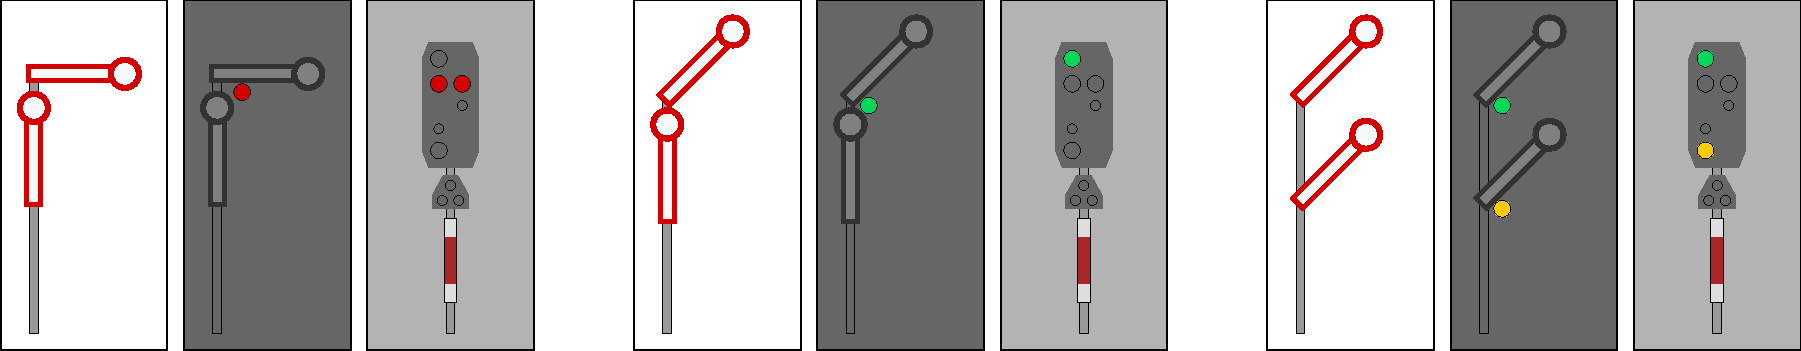
\includegraphics[width=420pt]{img/hp012.pdf}
%	\caption{from left to right: Hp0, Hp1, Hp2}
%	\label{fig:hp012}
%\end{figure} 

%\noindent

\layerOne{Other}

\layerTwo{git}

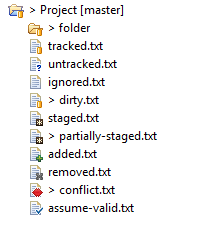
\includegraphics[width=120pt]{img/git-IconDecorations.png} %% von http://wiki.eclipse.org/EGit/User_Guide

\begin{itemize}
  \item \textbf{dirty (folder)} - At least one file below the folder is dirty; that
  means that it has changes in the working tree that are neither in the index nor in the repository.
  \item \textbf{tracked} - The resource is known to the Git repository and hence
  under version control.
  \item \textbf{untracked} - The resource is not known to the Git repository
  and will not be version controlled until it is explicitly added.
  \item \textbf{ignored} - The resource is ignored by the Git team provider. The
  preference settings under Team $>$ Ignored Resources, "derived" flag and
  settings from .gitignore files are taken into account.
  \item \textbf{dirty} - The resource has changes in the working tree that are
  neither in the index nor in the repository.
  \item \textbf{staged} - The resource has changes which have been added to the
  index. Note that adding changes to the index is currently possible only in the commit dialog via the context menu of a resource.
  \item \textbf{partially-staged} - The resource has changes which are added to the
  index and additional changes in the working tree that neither reached the index nor have been committed to the repository. See partial staging from the Git Staging view for how to do that.
  \item \textbf{added} - The resource has not yet reached any commit in the
  repository but has been freshly added to the Git repository in order to be tracked in future.
  \item \textbf{removed} - The resource is staged for removal from the Git
  repository.
  \item \textbf{conflict} - A merge conflict exists for the file.
  \item \textbf{assume-valid} - The resource has the "assume unchanged" flag. This
  means that Git stops checking the working tree files for possible modifications, so you need to manually unset the bit to tell Git when you change the working tree file. Also see Assume unchanged action.
\end{itemize}

\layerThree{fetch}

Fetch from remote repository

\layerThree{pull}

Incorporates changes from a remote repository into the current branch. 
In its default mode, git pull is shorthand for git fetch followed by git merge FETCH_HEAD.

\layerThree{commit}

Commit changes to local repository

\layerThree{push}

Push Commits to remote repository

\layerThree{conflicts}

\url{http://wiki.eclipse.org/EGit/User_Guide#Resolving_a_merge_conflict}

\layerThree{branches}
branch
merge
rebase
cherry-pick

\layerThree{revert}

If a commit which has not yet been pushed has to be undone:

Select folder \rightMouse Team \rightArrow Show in History \\
Note number of commit
\\ then use command line \\
{\ttfamily git revert <noted number>}

\vspace{5mm}
\noindent If a commit which has already been pushed has to be undone:

Is done the same way.

\vspace{5mm}
\noindent Note: Both reverts don't undo history. The wrong commit and the reversion will
be logged.

\layerOne{Literature}

\begin{itemize}
  \item A Unifying Approach to Connections for Multi-Level Modeling
  \cite{article:AtkinsonGerbigKuehne2015}
  \begin{itemize}
  \item Melanie � Multi-level Modeling and Ontology Engineering
  Environment \cite{article:AtkinsonGerbig2012}
  \item Referenced 2
  \item Referenced 3
\end{itemize}
\end{itemize}

\nocite{article:test}

\layerOne{Weekly Reports}
\setcounter{section}{14}
\layerTwo{2015}
\setcounter{subsection}{36}

\layerThree{7 Sep 2015 - 11 Sep 2015}
\begin{itemize}
\item Made browser tabs closeable
\item Init Requirements and Specifications in LaTeX
\item Added Panic button to GUI
\item Image loading: XML file now derived from IMG file name and path instead of storing
that information in the IMG file.
\item Division of BigIntegers fixed, Multiplication of negative Integers fixed
\end{itemize}

\layerThree{14 Sep 2015 - 18 Sep 2015}
\begin{itemize}
\item Tested and documented some git features.
\item Produced conflicts in git: Managed to resolve them finally. It was challenging. Further
testing required.
\item Tried to install safari. Waiting for Help desk...
\item Made the browser work again. Several fixes: Removed layouter, changed locking mechanism,
set to native browser
\end{itemize}

\layerThree{21 Sep 2015 - 25 Sep 2015}
Used XMF to do exercises with meta-classes \begin{itemize} 
\item to understand the concept of class, object, instantiation and inheritance
\item to override the default meta-object-protocol, be redefining new/get/set etc.
\item to understand the default behaviour of XMF
\end{itemize}

\layerThree{28 Sep 2015 - 2 Oct 2015}
\begin{itemize} 
\item Continued experiments with meta-classes
\item Gathered ideas for website; some experiments with html.
\end{itemize}

\layerThree{5 Oct 2015 - 9 Oct 2015}
\begin{itemize} 
\item Preparation for discussions about intrinsics.
\item Fr: Travel
\end{itemize}

\layerThree{12 Oct 2015 - 16 Oct 2015}
\begin{itemize} 
\item Mo,Tu,Fr: holiday
\item Making documentation for sceanarios for changes on intrinsic attributes
\item Tiny bugfix in FormsClient
\end{itemize}

\layerThree{19 Oct 2015 - 23 Oct 2015}
\begin{itemize} 
\item Mo: Travel
\item Added Monospace (with anti-alias) font to editor window.
\end{itemize}

\layerThree{26 Oct 2015 - 30 Oct 2015}
\begin{itemize} 
\item Started to fix HTML generation
\end{itemize}

\layerThree{2 Nov 2015 - 6 Nov 2015}
\begin{itemize} 
\item Fixed Live Documentation
\item Drew diagram for intrinsics to verify current model
\end{itemize}

\layerThree{9 Nov 2015 - 13 Nov 2015}
\begin{itemize} 
\item fix syntax highlighting
\item fix \%20 at welcome page
\end{itemize}

\layerThree{16 Nov 2015 - 20 Nov 2015}
\begin{itemize} 
\item fix fonts, test change fonts dynamically
\item fix autocomplete . , ()
\item remove debug noDocFound, isLikelyToBeHTML
\end{itemize}

\layerThree{23 Nov 2015 - 27 Nov 2015}
\begin{itemize} 
\item Diagrams: added InstLevel to associations
\item fixed zoom
\end{itemize}

\layerThree{30 Nov 2015 - 3 Dec 2015}
\begin{itemize} 
\item Modified appearance of associations, added arrows
\item Added boxes for intrinsic Level
\item Multiplicity shows always
\end{itemize}

\layerThree{9 Dec 2015 - 10 Dec 2015}
\begin{itemize} 
\item Visit in Essen
\end{itemize}

\layerThree{14 Dec 2015 - 18 Dec 2015}
\begin{itemize} 
\item Changed label's and arrow's position on associations in diagrams
\item Tried to make DEL-key work in diagrams
\end{itemize}

\layerThree{ToDo}
\begin{itemize}
\item improve webpage
\item Specify FormClient, fix only
\item git commands in Eclipse
\item (nextWeek) MeMo language requirements
\item pw protected folder: \url{https://wincent.com/wiki/git_repository_access_control}
\item Snippets
\item look at/play with Kernel (Object/Class/Attribute)
%\item Use Notepad++ with syntax highlighting for user defined languages: \url{http://weblogs.asp.net/jongalloway/creating-a-user-defined-language-in-notepad}
\item HTMLViewer.xmf: Are ".o", ".xip", ".xto", ".xtd", ".xtml" still in use?
Welcome.xmf: requestURL ...
requirements
\item welcome page does not work in linux
\item experiment: call java function
%\item fix documentation bug (over lunch)
\item rectangular edges only on some edge types
\item Show/hide in Diagram

\end{itemize}


\clearpage
\phantomsection
\addcontentsline{toc}{chapter}{Bibliography}
\bibliography{literature}
\bibliographystyle{literatureStyle}
\end{document}
